\documentclass[conference]{IEEEtran}
\IEEEoverridecommandlockouts
% The preceding line is only needed to identify funding in the first footnote. If that is unneeded, please comment it out.
\usepackage{cite}
\usepackage{hyperref}
\usepackage{amsmath,amssymb,amsfonts}
\usepackage{algorithmic}
\usepackage{graphicx}
\usepackage{textcomp}
\usepackage{xcolor}
\def\BibTeX{{\rm B\kern-.05em{\sc i\kern-.025em b}\kern-.08em
    T\kern-.1667em\lower.7ex\hbox{E}\kern-.125emX}}
\begin{document}

\title{Implementing Deep Learning Models for Enhancing Bluetooth-based Localization Algorithms*\\
{\footnotesize \textsuperscript{*}Advances in Indoor Localization Using Deep Learning Techniques}
\thanks{Identify applicable funding agency here. If none, delete this.}
}

\author{\IEEEauthorblockN{1\textsuperscript{st} Camilo Leuro}
\IEEEauthorblockA{\textit{dept. Ciencias de la Computación e IA} \\
\textit{Universidad Sergio Arboleda}\\
Bogotá, Colombia \\
camilo.leuro01@usa.edu.co}
\and
\IEEEauthorblockN{2\textsuperscript{nd} Carolay Camacho-Sanchez}
\IEEEauthorblockA{\textit{dept. Ciencias de la Computación e IA} \\
\textit{Universidad Sergio Arboleda}\\
Bogotá, Colombia \\
carolay.camacho01@usa.edu.co}
\and
\IEEEauthorblockN{3\textsuperscript{rd} Andrés García}
\IEEEauthorblockA{\textit{dept. Ciencias de la Computación e IA} \\
\textit{Universidad Sergio Arboleda}\\
Bogotá, Colombia \\
andres.garcia13@usa.edu.co}
\and
\IEEEauthorblockN{4\textsuperscript{th} Mateo Rondon}
\IEEEauthorblockA{\textit{dept. Ciencias de la Computación e IA} \\
\textit{Universidad Sergio Arboleda}\\
Bogita, Colombia\\
mateo.rondon01@usa.edu.co}
}

\maketitle

\begin{abstract}
ndoor localization remains a formidable challenge in the absence of reliable GPS signals. This study tackles this issue by harnessing advanced Deep Learning techniques. We leverage the UJIIndoorLoc dataset to construct a WLAN fingerprint-based model, executed within a Python programming framework following the CRISP-DM methodology. Our findings underscore the pivotal role of deep learning in addressing the intricate challenges of indoor localization, offering promising solutions for real-world applications.
\end{abstract}

\begin{IEEEkeywords}
Indoor localization, UJIIndoorLoc, Wireless fingerprinting, Data analysis.
\end{IEEEkeywords}

\maketitle


\section{Introduction}
The relentless progress of technology continually shapes and redefines our interaction with the world around us. Amidst the spectrum of technological evolutions, the realm of localization, particularly indoor localization, has emerged as a pivotal aspect. Be it for assisting individuals in vast shopping malls, ensuring patient safety in sprawling hospitals, or aiding travelers in international airports, accurate indoor localization can revolutionize experiences in myriad ways.

Historically, the quest for impeccable indoor localization has seen a gamut of solutions, ranging from infrared to ultrasonic sensors. Yet, each came with its own set of limitations, often tethered by accuracy, infrastructure costs, or scalability. The ubiquity of Global Positioning System (GPS), while transformative for outdoor localization, falters within the confines of concrete walls and metal structures, rendering it inefficient for indoor scenarios\textcolor{blue}{\cite{zhang2013comprehensive}}.

In this milieu, the rise of Deep Learning, with its adeptness at deciphering patterns from vast datasets, offers a glimmer of hope. Renowned for reshaping domains from natural language processing to computer vision, its application to indoor localization promises potential breakthroughs\textcolor{blue}{\cite{alsheikh2015deep}}. Motivated by this, our study embarks on an exploration of harnessing Deep Learning for indoor localization, leveraging the rich data from the UJIIndoorLoc dataset.

The adoption of the Cross-Industry Standard Process for Data Mining (CRISP-DM) in our investigation underscores its significance in guiding data-driven endeavors. Recognized for its structured approach in the data mining process, CRISP-DM provides a comprehensive framework that ensures systematic exploration, analysis, and interpretation of datasets. By harnessing its methodologies, we aspire to navigate the intricacies of the UJIIndoorLoc dataset effectively, ensuring a rigorous and holistic understanding of indoor localization dynamics.

With this endeavor, we aspire not merely to navigate the intricacies of indoor localization but also etch a significant mark in the evolving narrative of Deep Learning applications.

In this study, we explore the application of advanced Deep Learning techniques to address the intricate challenges of indoor localization. Our specific objectives include:

\begin{enumerate}
\item Constructing a WLAN fingerprint-based model using the UJIIndoorLoc dataset.
\item Implementing the research within a Python programming framework.
\item Following the CRISP-DM methodology to ensure a structured and comprehensive approach.
\item Highlighting the pivotal role of Deep Learning in offering promising solutions to the challenges of indoor localization.
\end{enumerate}


\section{Literature Review}

In recent years, the field of indoor localization has gained significant attention, with several studies exploring various methodologies to optimize the accuracy and efficiency of indoor positioning systems. One notable contribution in this domain is the work by Terán and Ore (2019), who performed a benchmark analysis of different algorithms for determining user indoor positioning utilizing the UJIIndoorLoc dataset \textcolor{blue}{\cite{teran2019benchmark}}. Their comprehensive study provided insights into the strengths and limitations of various algorithms, setting a foundational understanding of the dataset's potential for indoor localization.

Continuing with the exploration of indoor localization through WiFi fingerprinting, numerous studies have delved into the application of deep learning techniques. Alsheikh et al. (2015) discussed the potential of deep learning in wireless localization tasks, highlighting its ability to model complex relationships and enhance the positioning accuracy\textcolor{blue}{\cite{alsheikh2015deep}}. This work underscores the versatility of deep learning methods in addressing the challenges inherent in indoor localization scenarios.

Furthermore, the comprehensive review by Zhang et al. (2013) sheds light on the diverse range of technologies and methodologies employed for indoor localization\textcolor{blue}{\cite{zhang2013comprehensive}}. The authors meticulously analyzed the evolution of indoor positioning systems, emphasizing the limitations of technologies such as infrared and ultrasonic sensors and highlighting the potential of emerging methodologies.

Collectively, these studies underscore the dynamic nature of indoor localization research, illustrating the continuous advancements and the diverse array of methodologies being explored. The insights derived from these works provide a robust foundation for our study, guiding our exploration of harnessing deep learning for indoor localization using the UJIIndoorLoc dataset.

\section{Dataset Description}

The dataset under scrutiny is the \textbf{UJIIndoorLoc}, meticulously curated by Joaquín Torres-Sospedra and collaborators\cite{UJIIndoorLocPap}. This dataset offers a deep dive into the realm of indoor positioning systems, primarily focusing on WLAN fingerprinting or WiFi Fingerprinting. Created based on data captured in 2013 from 3 buildings with 3 and 4 floors of the Universitat Jaume I, it embodies the nuances and intricacies of indoor localization.

A holistic breakdown of its components is as follows:

\begin{itemize}
\item \textbf{Attributes 001 to 520 (WAP001-WAP520):} These delineate the intensity values from various Wireless Access Points (WAP). The values extend from $-104$ to $0$ and $+100$. It's noteworthy that a positive value of $100$ indicates non-detection of the WAP.
\item \textbf{Longitude:} Represents longitudinal coordinates, varying from -7695.9387549299299000 to -7299.786516730871000.
\item \textbf{Latitude:} Parallelly, latitude coordinates span from 4864745.7450159714 to 4865017.3646842018.
\item \textbf{Floor:} Specifies the altitude in terms of the building's floors, capturing integer values between 0 to 4.
\item \textbf{BuildingID:} A categorical indicator segregating the buildings. It assumes integer values from 0 to 2.
\item \textbf{SpaceID:} A categorical value illustrating the precise space (be it an office, corridor, classroom) of data capture.
\item \textbf{RelativePosition:} Portrays the positional nuance concerning the space, either being inside (1) or outside in front of the door (2).
\item \textbf{User ID, PhoneID, and Timestamp:} These attributes offer additional metadata about the user, the Android device used for data collection, and the exact UNIX timestamp of the data capture, respectively.
\end{itemize}

In terms of data typology, all attributes are instantiated as int64, barring longitude and latitude, which are represented as float64.

The \textbf{UJIIndoorLoc} dataset is a paragon in the sphere of indoor positioning. In light of the hitches posed by GPS systems in interior spaces due to architectural barriers, the gravity of precise indoor positioning stands unparalleled. Harnessing the unique signatures of proximate WiFi access points (WAPs) for device localization, this dataset accentuates the prowess of WiFi fingerprinting. The gamut of data, spanning WAP intensities, precise geospatial data, floor details, and building categorization, fortifies the dataset's primacy in advancing accurate indoor positioning—rendering it indispensable for aficionados and trailblazers in the field.

\section{Data Processing and Analysis}

In order to derive meaningful insights from the \textbf{UJIIndoorLoc} dataset, meticulous data processing and analysis were conducted. This encompassed preprocessing, exploratory data analysis, feature selection, and model implementation, ensuring that the data was molded into a format apt for high-quality insights.

\begin{enumerate}
\item \textbf{Preprocessing:} Initial procedures included managing missing data, normalizing intensity values to bring them onto a common scale, and encoding categorical variables. The aim was to refine the dataset by addressing any inconsistencies or discrepancies, setting it up for further analysis.


\item \textbf{Exploratory Data Analysis (EDA):} This phase sought to uncover underlying patterns, correlations, and outliers in the dataset. Visualization techniques and statistical approaches were utilized to understand the dataset's attributes, illuminating key elements for subsequent feature selection.

\item \textbf{Feature Selection:} Based on the revelations from the EDA, essential features were chosen to enhance the model's efficiency. This step concentrated on diminishing dimensionality, removing superfluous or redundant features, and preserving those with significant contributions to the model's predictive prowess.

\item \textbf{Model Implementation:} After feature selection, a variety of machine learning models were trialed and assessed based on their performance indicators. The best-performing model was further refined and validated to ensure it aptly captured the intricacies of indoor positioning.
\end{enumerate}

By systematically navigating through these phases, the \textbf{UJIIndoorLoc} dataset was elevated to a powerful instrument, primed to decode the complexities of indoor positioning. The refined dataset, equipped with enhanced features and a formidable model, showcases the progress in indoor positioning technologies and stands as a pivotal resource for ongoing research and advancements in the sector.



\subsection{Description of the CRISP Methodology}
\label{sec:metodo_crisp}

The Cross Industry Standard Process for Data Mining (CRISP-DM) served as the foundational methodology guiding our exploration of the \textbf{UJIIndoorLoc} dataset. This iterative process consists of six essential stages, which were meticulously applied and adapted to the intricacies of indoor positioning data. The stages and their specific applications to our dataset are described below:

\begin{enumerate}
    \item \textbf{Understanding the Business:} At this stage, our primary objective was to comprehend the challenges associated with indoor positioning, especially in environments where GPS signals are ineffective. Our goal was to harness the capabilities of the \textbf{UJIIndoorLoc} dataset to address these challenges.
    
    \item \textbf{Understanding the Data:} A comprehensive exploration of the dataset was conducted, discerning attributes like intensity values from different WAPs, geospatial data, floor numbers, and building identifiers. This step was crucial to appreciate the dataset's potential in addressing indoor positioning needs.
    
    \item \textbf{Data Preparation:} The data was scrutinized for missing values, inconsistencies, and discrepancies. Intensity values were normalized, and categorical variables, such as the BuildingID, were appropriately encoded to prepare the dataset for modeling.
    
    \item \textbf{Modeling:} Based on the insights from the preliminary stages, several machine learning models were implemented. These models aimed to exploit the dataset's features to predict precise indoor positions.
    
    \item \textbf{Evaluation:} Each model's performance was rigorously assessed against predefined metrics. This evaluation was crucial in selecting the most suitable model that aligned with our business objectives and delivered optimal results for indoor positioning.
    
    \item \textbf{Implementation:} The finalized model was integrated into a suitable platform, ensuring that stakeholders could seamlessly access and utilize the results for their specific indoor positioning needs.
\end{enumerate}

By adhering to the CRISP-DM methodology, we ensured a systematic and thorough exploration of the \textbf{UJIIndoorLoc} dataset, transforming it into a valuable tool for advancing indoor positioning technologies.

\section{Visual Representation of Findings}

In this section, we delve into the UJIIndoorLoc dataset's graphical interpretations. By highlighting the specifics of WLAN fingerprinting and indoor positioning through visuals, we endeavor to bring forth patterns, correlations, and key details that might elude textual or tabular formats. Presented hereafter are a collection of visual results, each revealing distinct aspects of our detailed examination.



\begin{figure}[h!]
    \centering
    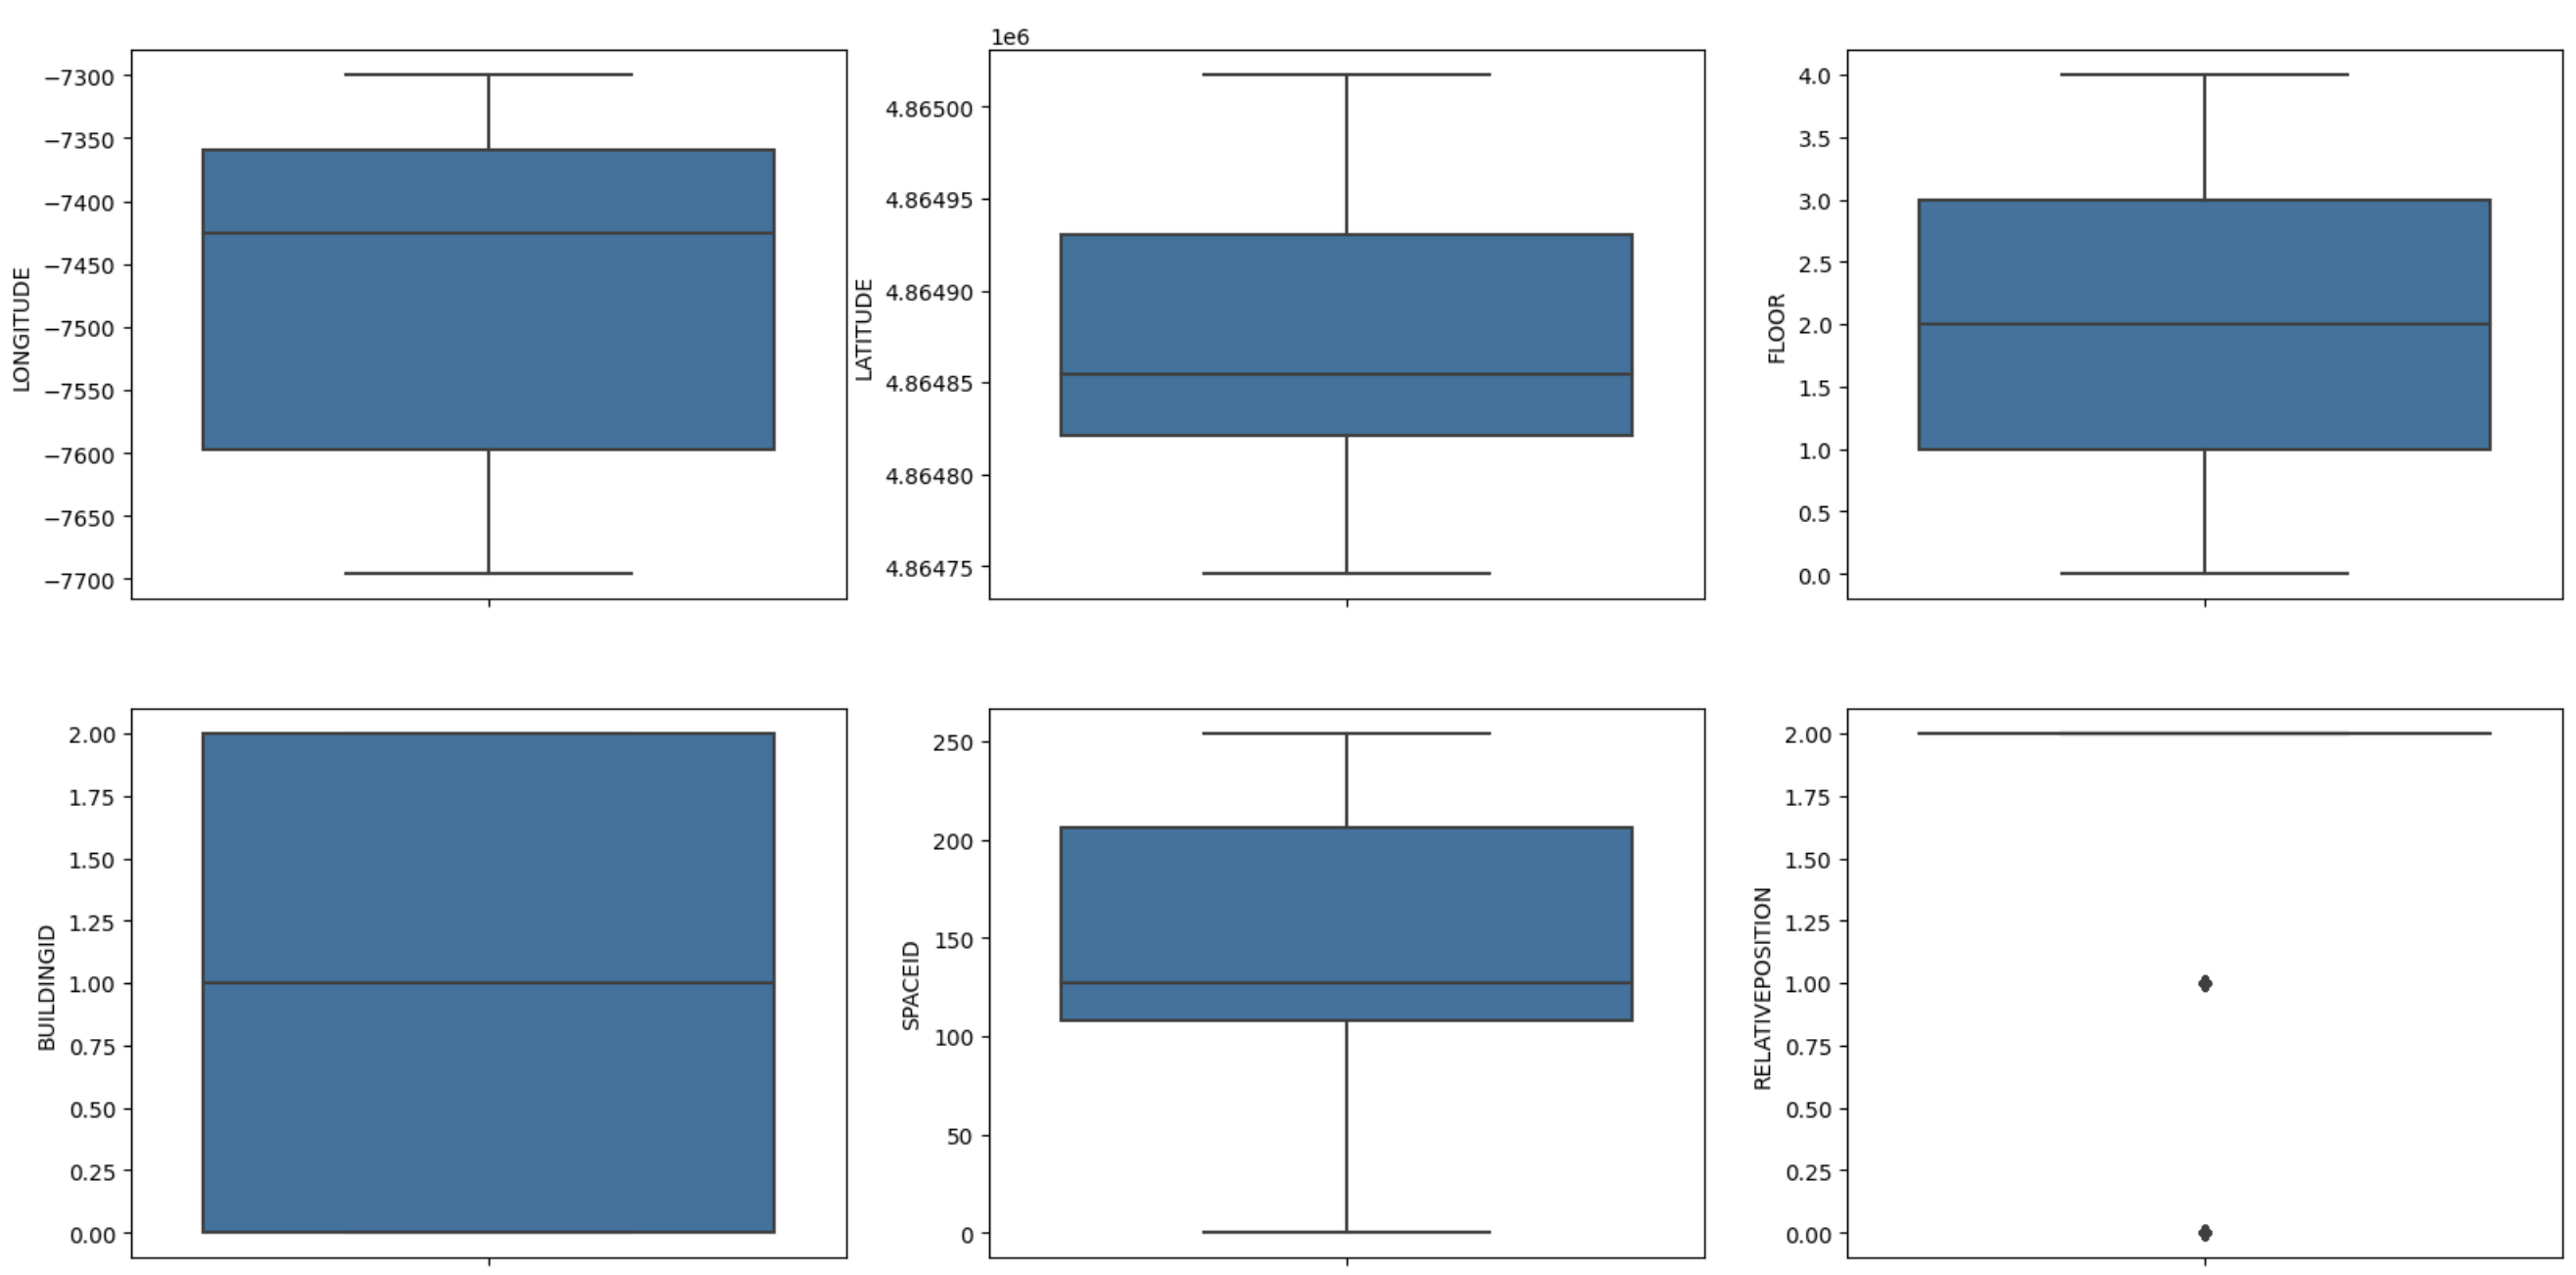
\includegraphics[width=0.5\linewidth]{Images/Figure1.png}
    \caption{Box plots for selected attributes from the UJIIndoorLoc dataset}
    \label{fig:boxplots}
\end{figure}


Figure 1 From these box plots, it is evident that within the non-intensity measurement columns, no outliers or atypical data points are observed.


\begin{figure}[h!]
    \centering
    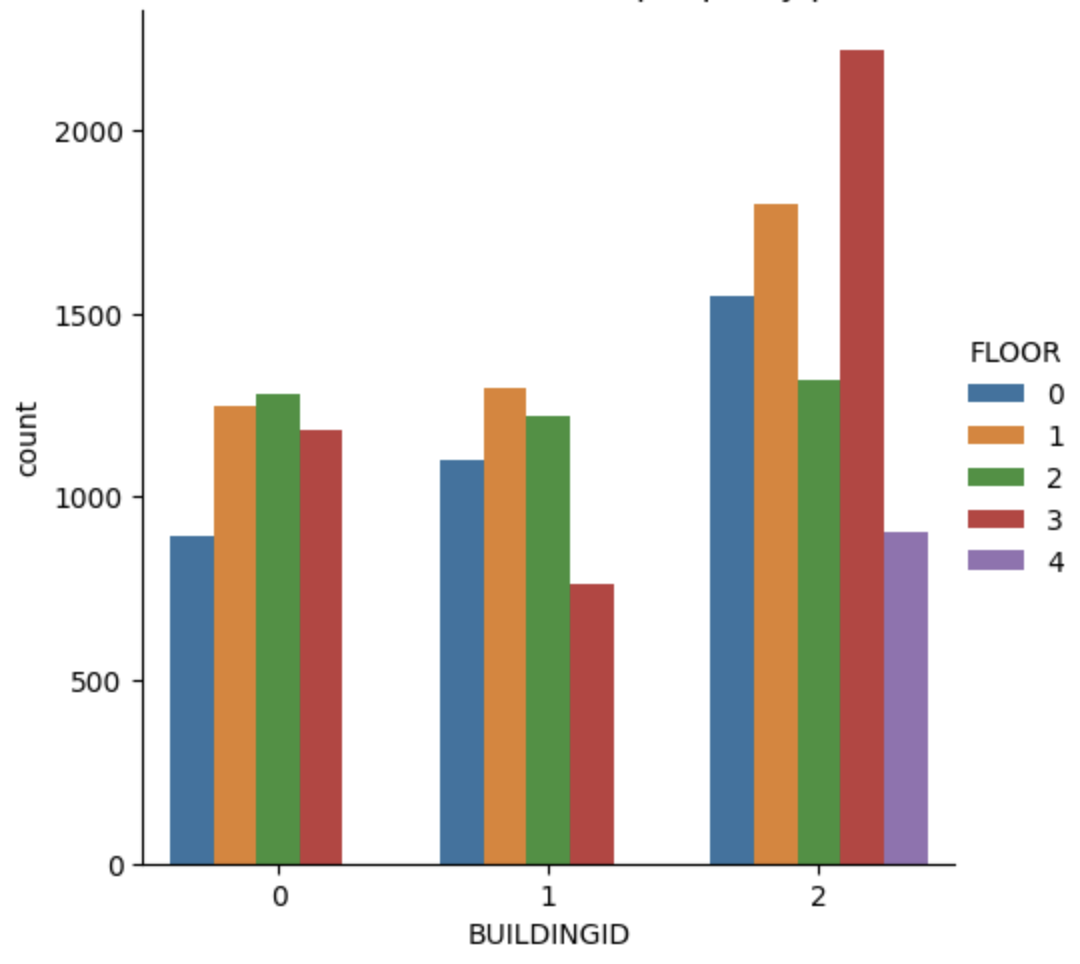
\includegraphics[width=0.5\linewidth]{Images/Imagen2.png}
    \caption{Quantity of data collected per floor and per building}
    \label{fig:enter-label}
\end{figure}


As observed in Figure 2, only one building has measurements on the 4th floor, while the others lack this, possibly due to the absence of a fourth floor.

\begin{figure}[h!]
    \centering
    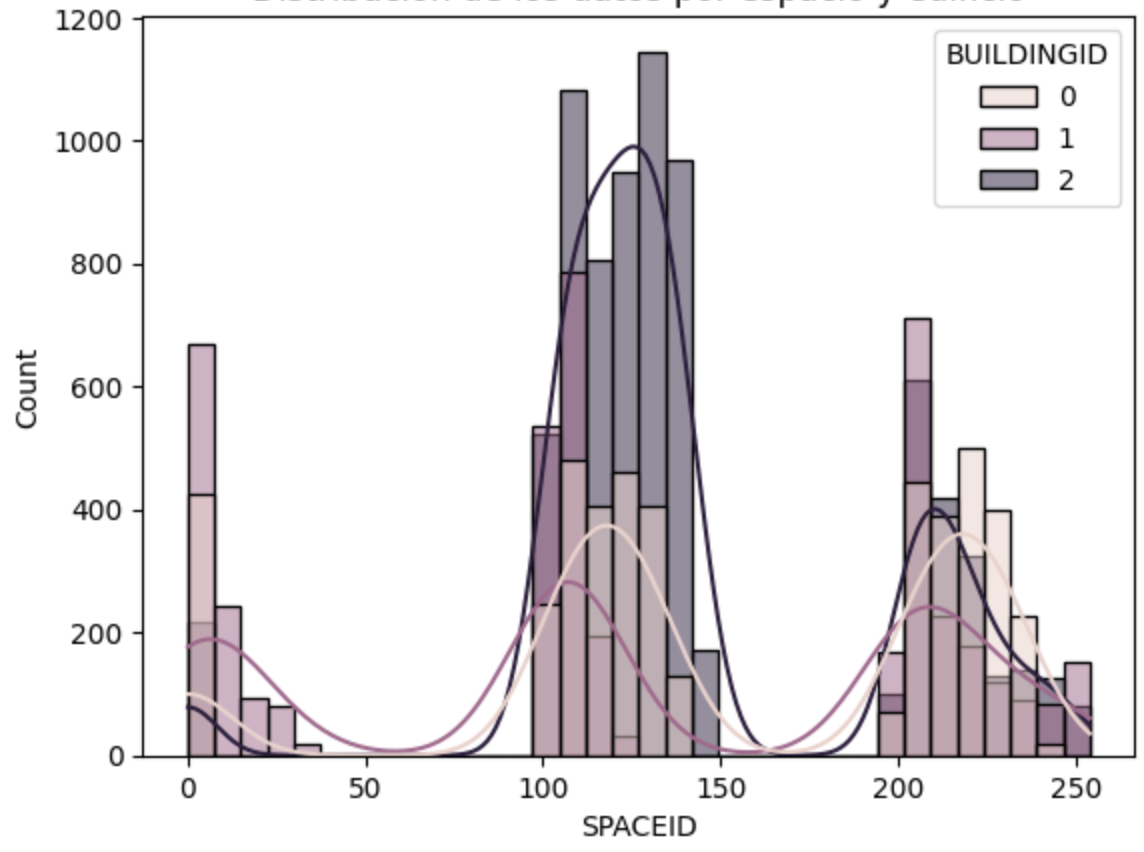
\includegraphics[width=0.5\linewidth]{Images/Image3.png}
    \caption{Distribution of data by space and building}
    \label{fig:enter-label}
\end{figure}

As depicted in Figure 3, the majority of data points are concentrated between spaces 100 to 150, with the second most prominent range being spaces 200 to 250. There is no linear categorization of spaces.


\begin{figure}[h!]
    \centering
    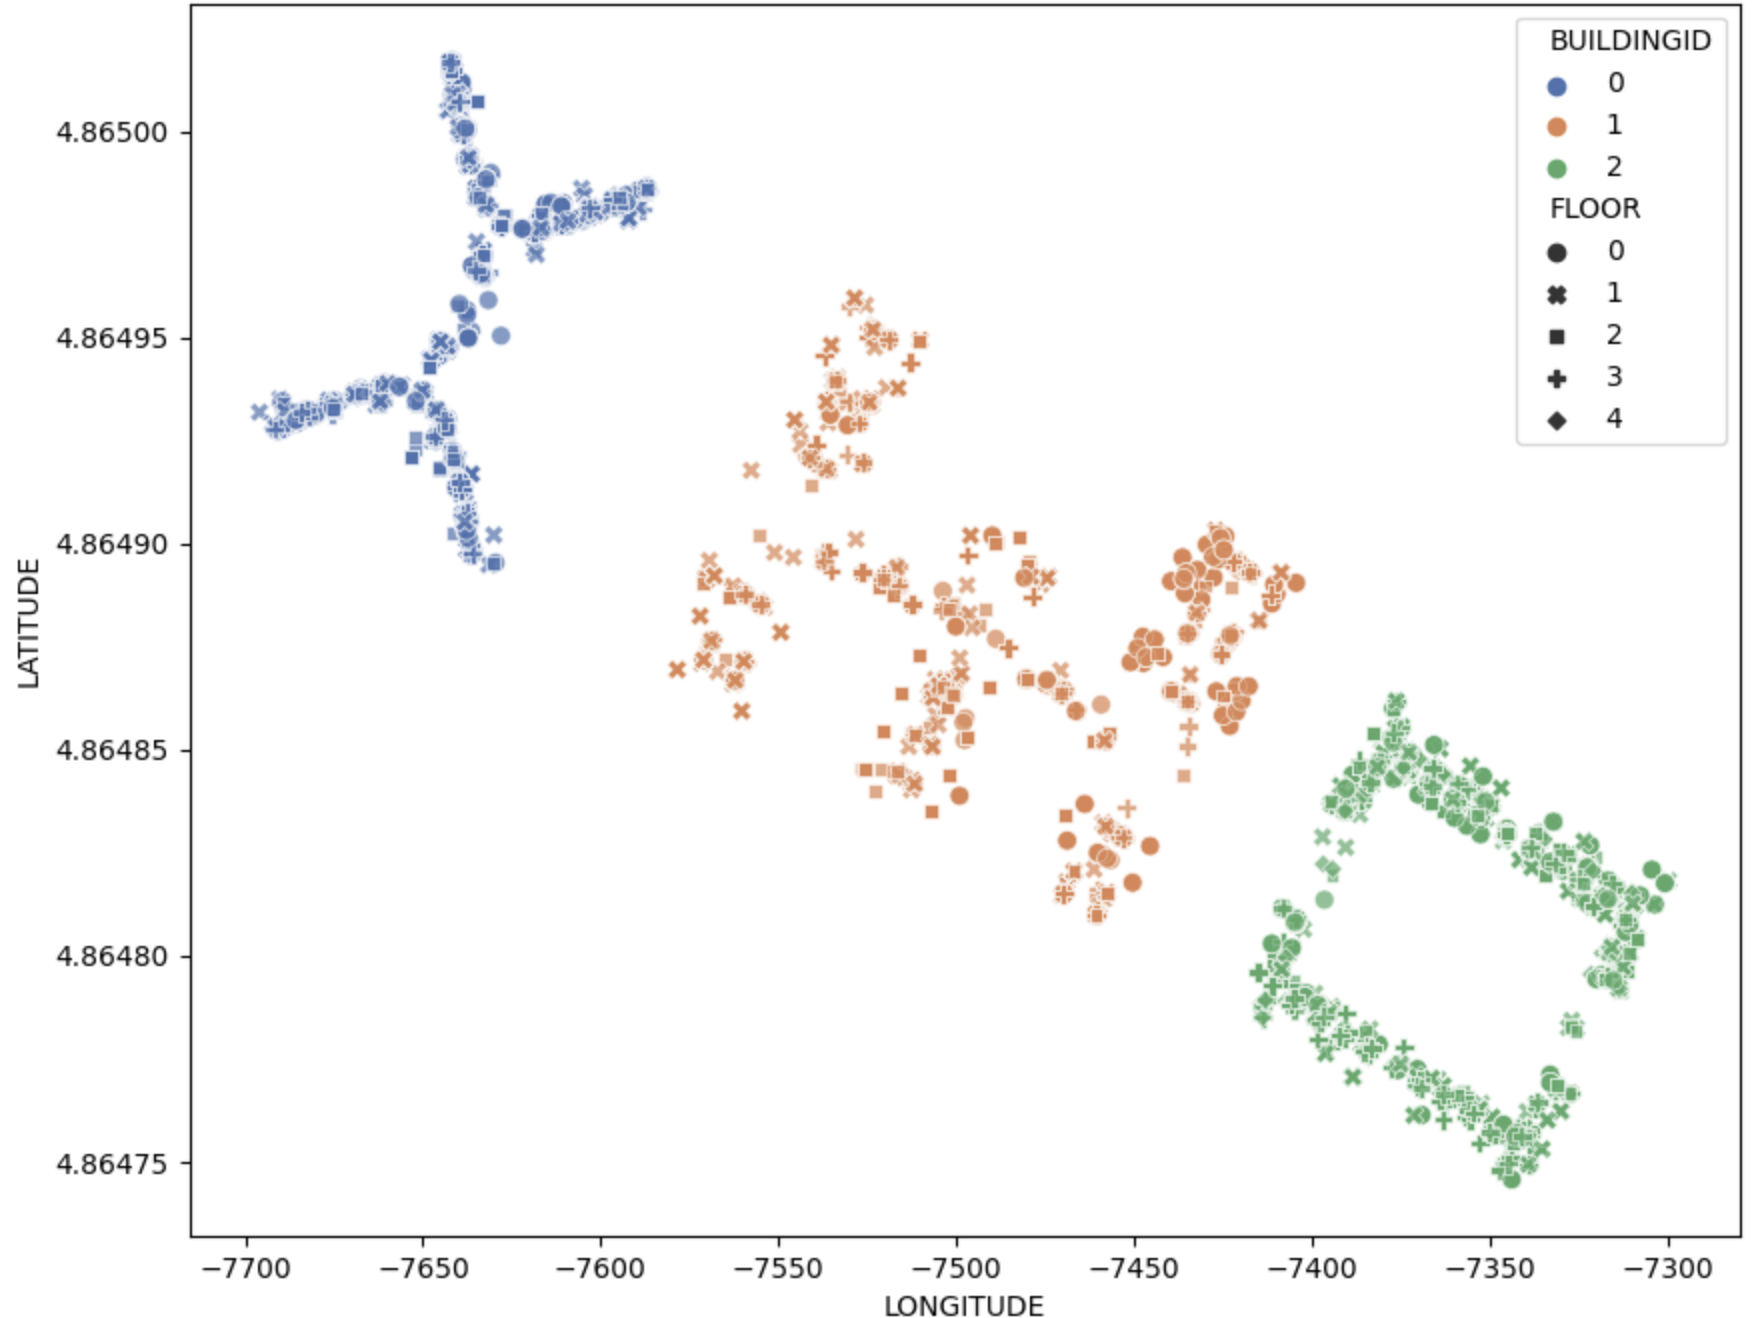
\includegraphics[width=0.5\linewidth]{Images/Figure4.png}
    \caption{Geographical Distribution of Measurements by Building and Floor}
    \label{fig:enter-label}
\end{figure}


Then, we created a series of heatmaps to visualize the average signal strength of Wireless Access Points (WAPs) across different floors. Each heatmap represents a specific floor, with columns corresponding to individual WAPs. The color scale indicates signal intensity (in dBm), where warmer colors signify stronger signals.

Notably, on the 4th floor, many attributes exhibit an average value of 100, primarily because only one building in the dataset has 4 floors. This renders several WAPs irrelevant for this floor's measurements.

Moreover, when examining specific WAPs (e.g., WAP205 to WAP221), it becomes apparent that they have limited measurements across all 4 floors, suggesting their potential insignificance for the indoor positioning model due to sparse data.

\begin{figure}[h!]
    \centering
    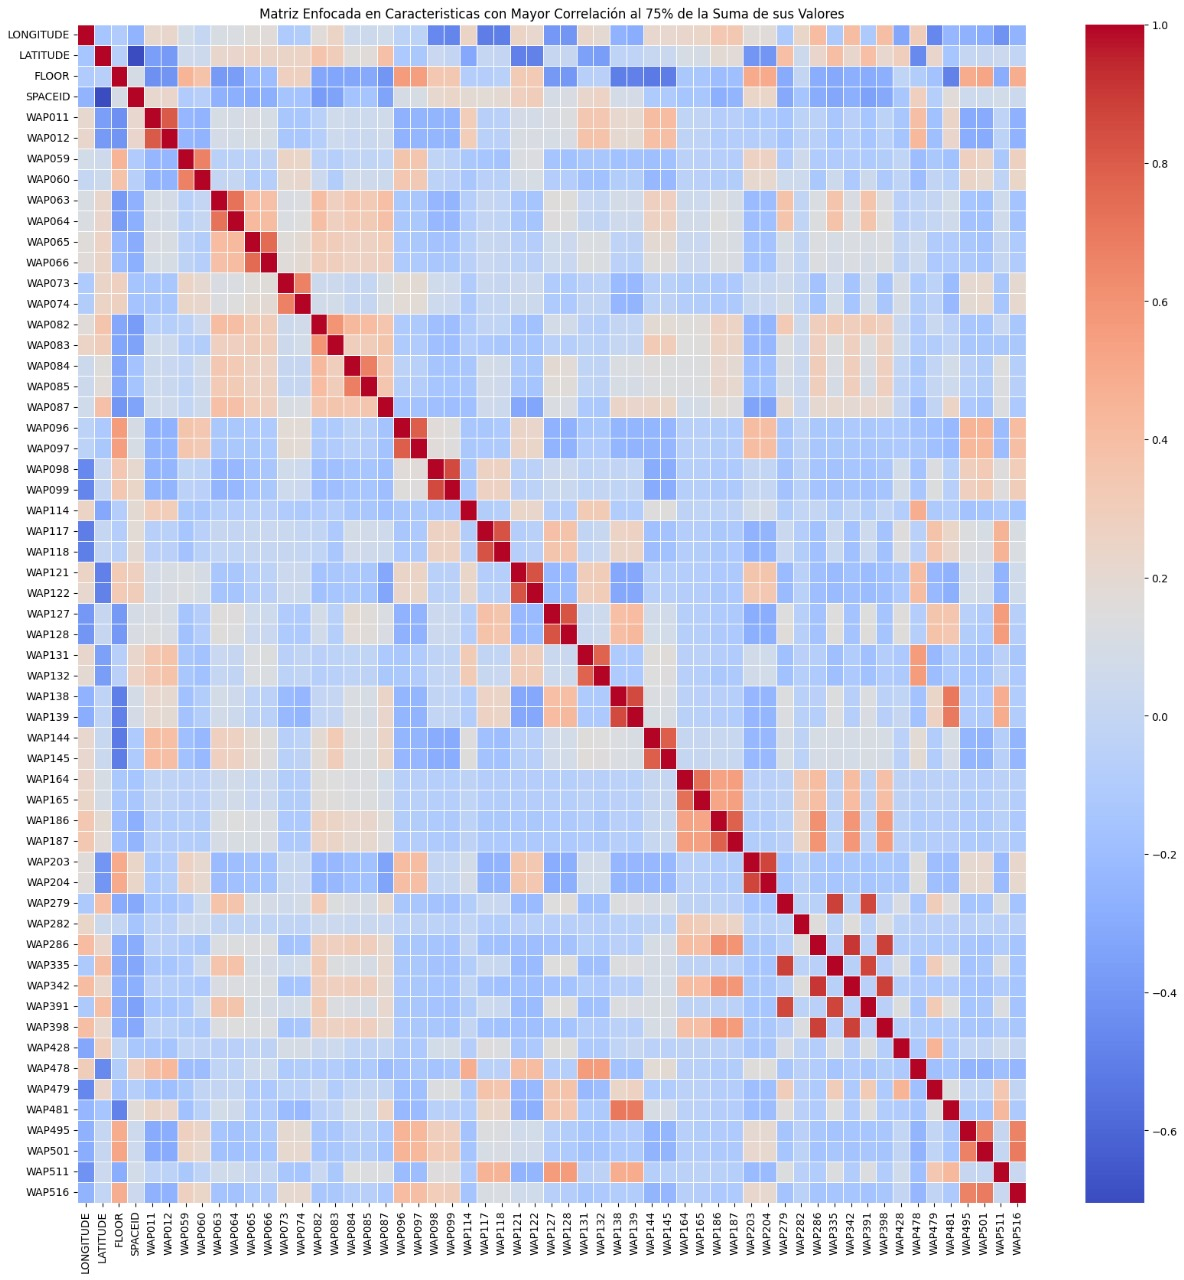
\includegraphics[width=0.5\linewidth]{Images/Imagecorrelacion.jpeg}
    \caption{Focused Matrix on Features with Higher Correlation to the Mean Sum of their Values}
    \label{fig:enter-label}
\end{figure}



Also, we constructed a correlation matrix to assess relationships between dataset attributes. The heatmap visualizes correlations, with warmer hues indicating positive correlations and cooler hues indicating negative ones. While numerical annotations are omitted for simplicity, this visualization helps identify potential patterns and associations among variables.

To narrow down our feature set for modeling, we identified columns whose cumulative correlations with other variables exceeded the average sum of all such correlations. This approach retains attributes likely to provide significant contributions to our model.

This process reduced the dataset to a subset of columns, streamlining data for modeling while maintaining data quality and relevance. The resulting dataset contains fewer columns, enhancing model development feasibility and potential accuracy for indoor positioning.


Next, we narrow our focus to a single building for in-depth analysis. We utilize box plots to visualize the distribution of selected attributes within this building. These box plots help us identify any outliers or atypical data points, particularly in non-intensity measurement columns. Fortunately, no such outliers were found in these columns.

We proceed by examining the distribution of data points across different spaces within the chosen building using a histogram. The histogram reveals that the majority of data points are concentrated within spaces numbered from 100 to 150, with the next most prominent range being spaces from 200 to 250. This distribution demonstrates the absence of a linear categorization for these spaces.

Additionally, we visualize the geographical distribution of measurements within the selected building and across different floors. The scatterplot offers insights into the building's shape based on the recorded readings.

Subsequently, we reiterate the importance of feature selection based on cumulative correlations and discuss the reduction in the number of columns. 

\begin{figure}[h!]
    \centering
    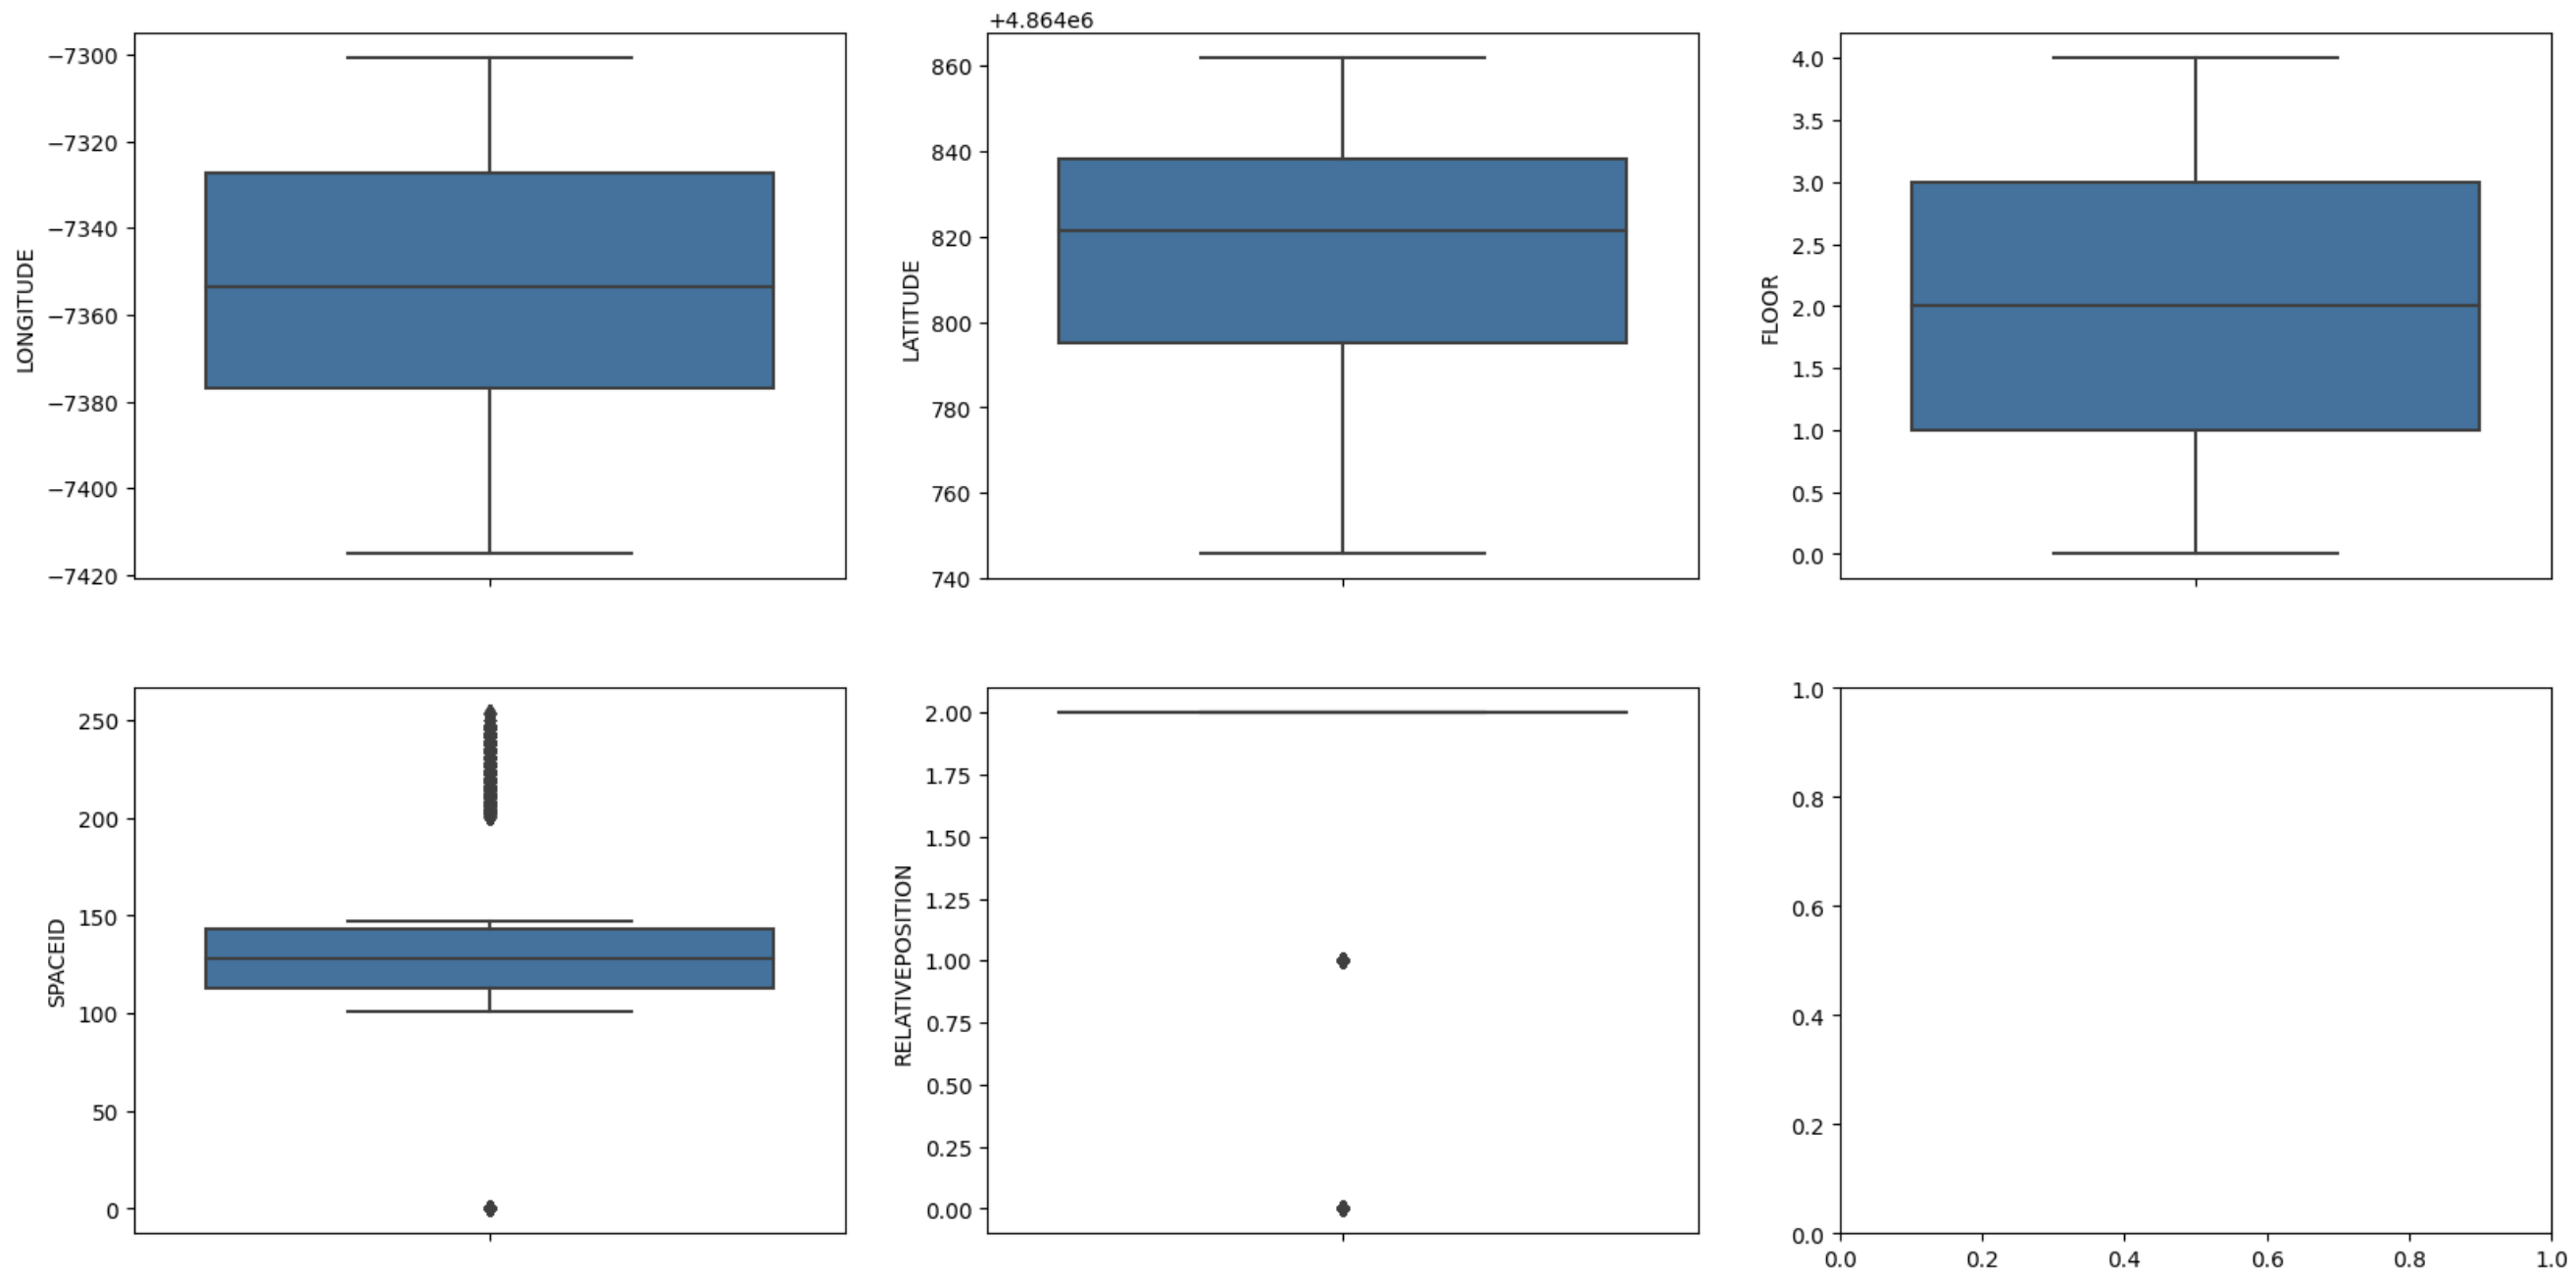
\includegraphics[width=0.5\linewidth]{Images/image5.png}
    \caption{Box Plots for Attribute Distribution}
    \label{fig:enter-label}
\end{figure}

\begin{figure}[h!]
    \centering
    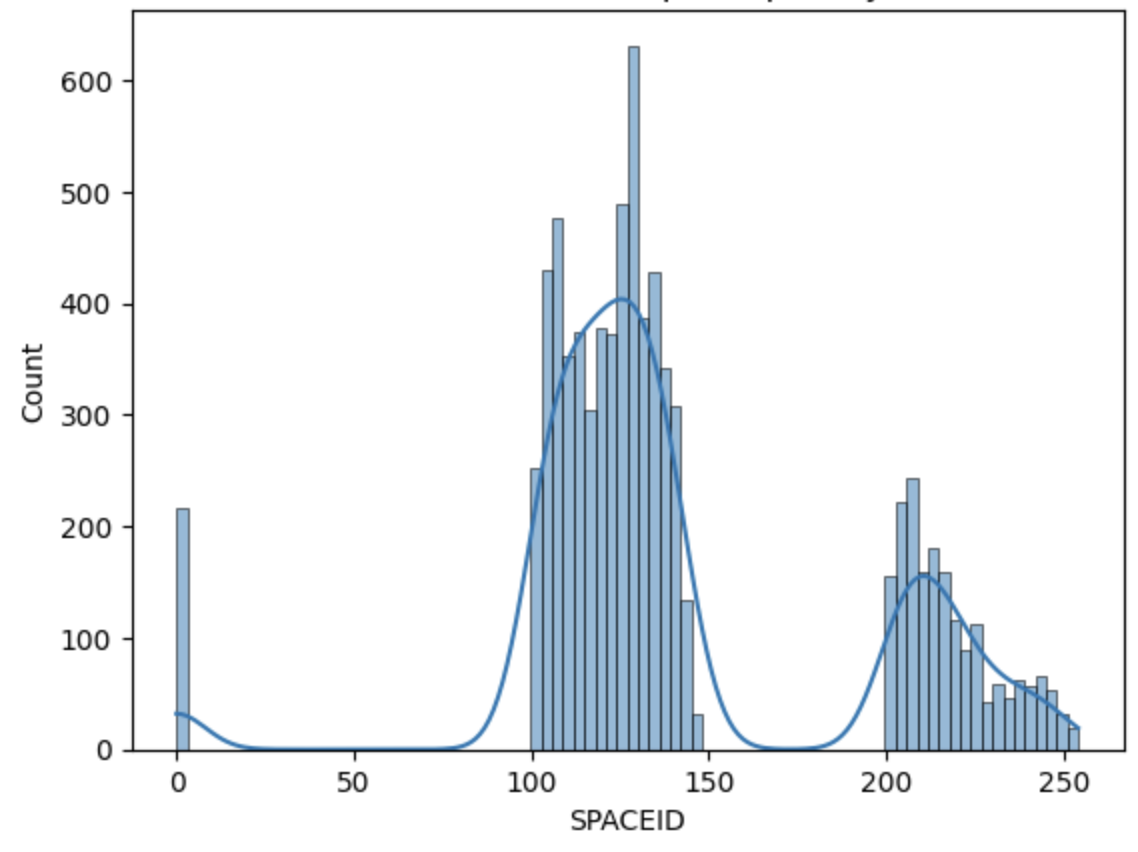
\includegraphics[width=0.5\linewidth]{Images/Image6.png}
    \caption{Data Distribution by Space and Building}
    \label{fig:enter-label}
\end{figure}

\begin{figure}[h!]
    \centering
    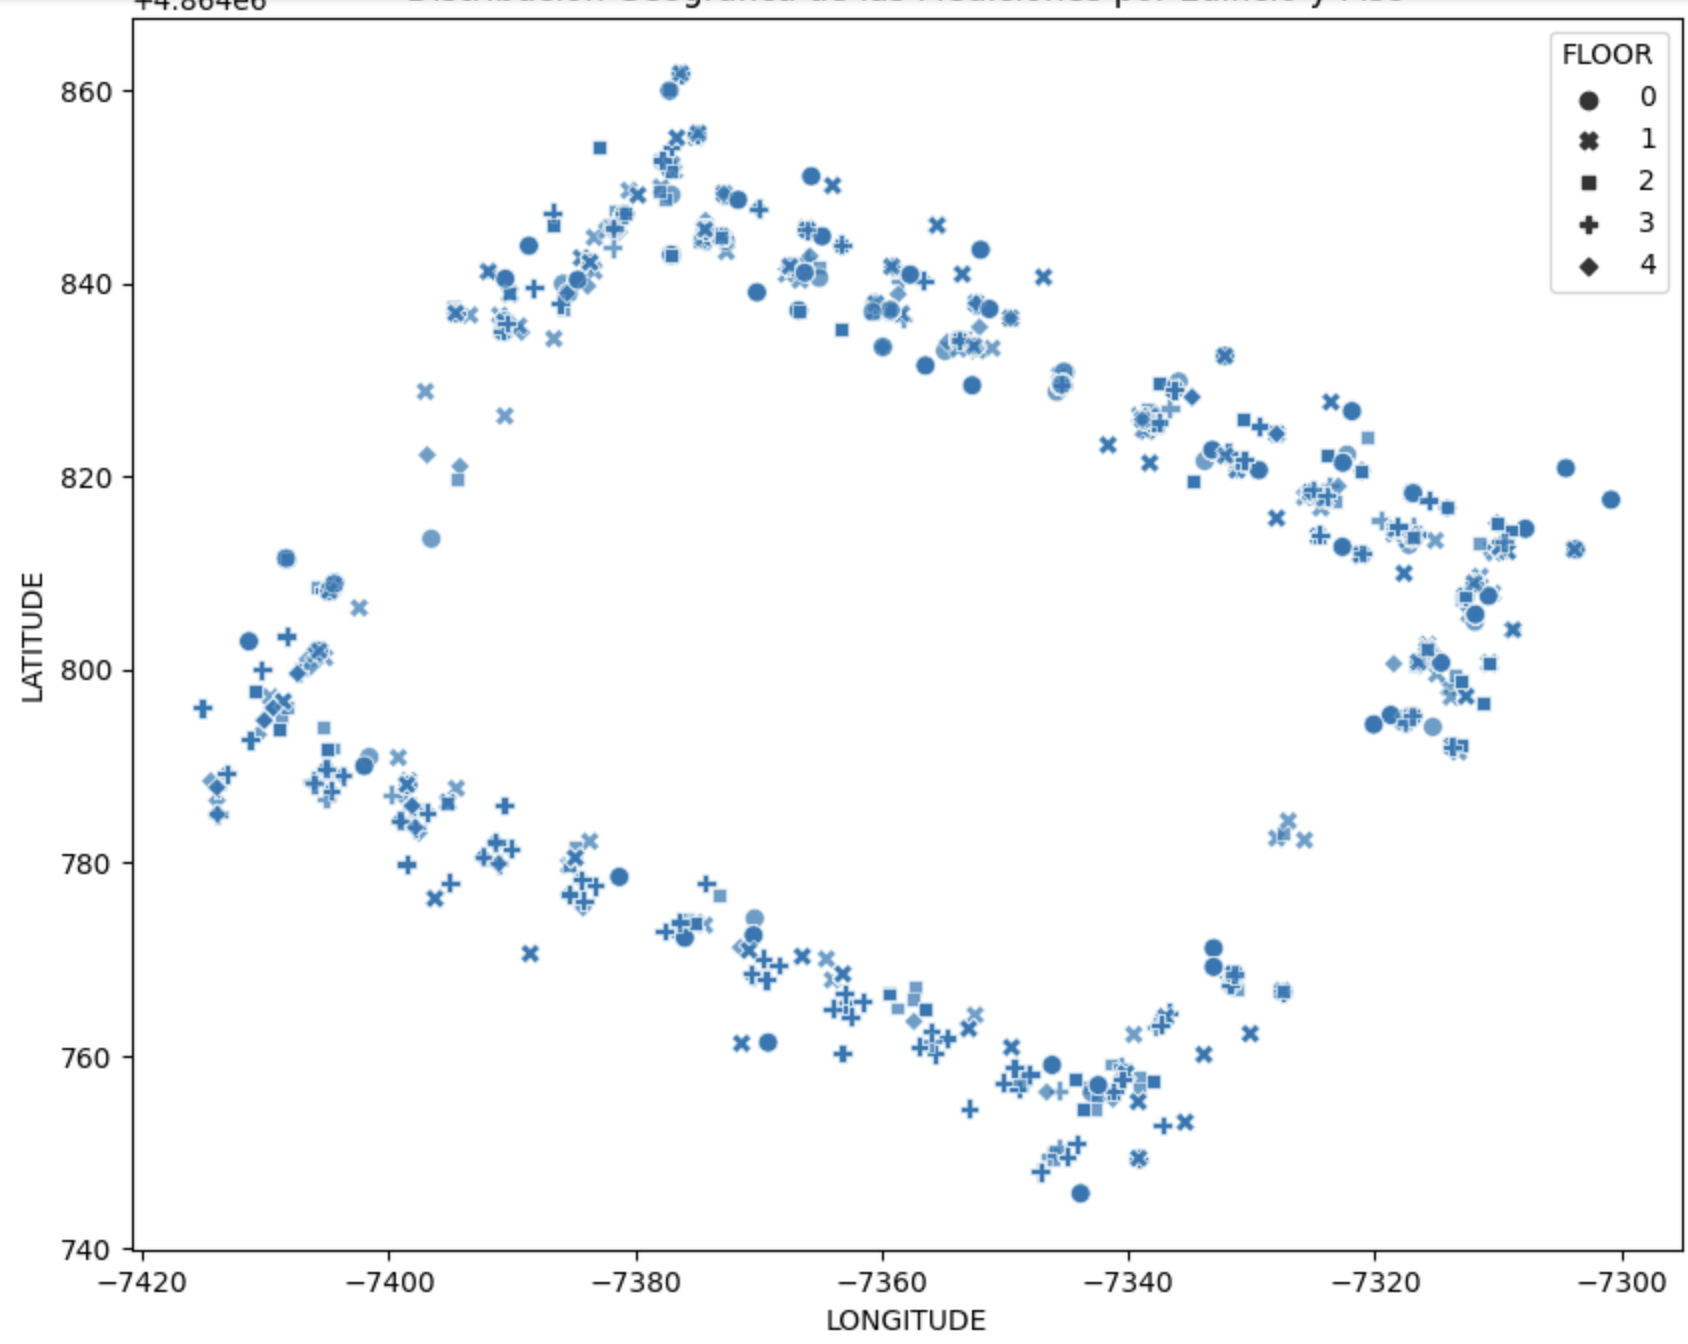
\includegraphics[width=0.5\linewidth]{Images/Image7.png}
    \caption{Geographical Measurement Distribution}
    \label{fig:enter-label}
\end{figure}


Finally, data normalization is performed using standard scaling, resulting in a standardized dataset for model development. This normalization process ensures that all variables have similar scales, enhancing model performance and interpretability.


\section*{Conclusion}

In this study, we embarked on a comprehensive exploration of the UJIIndoorLoc dataset, aiming to uncover valuable insights and patterns related to WLAN fingerprinting and indoor positioning. Through a meticulous analysis, we shed light on various aspects of the dataset, from data distributions and spatial characteristics to attribute relevance and correlations.

Our initial visual representations, as showcased in Figure 1, Figure 2, and Figure 3, allowed us to discern significant observations. We identified that only one building featured measurements on the 4th floor, suggesting the potential absence of a fourth floor in the other buildings. Additionally, our analysis revealed that data points were most concentrated between spaces 100 to 150, with spaces 200 to 250 ranking second in terms of prevalence. This non-linear categorization of spaces presents a noteworthy challenge in our modeling process.

Further analysis delved into attribute relevance and correlation. By analyzing correlation matrices and selecting attributes with a sum of correlations above the dataset average, we aimed to streamline our dataset. This process not only reduced memory usage but also improved the dataset's focus on the most informative features for building our indoor positioning model.

Lastly, we discussed the normalization of our data using standard scaling, preparing it for subsequent modeling and analysis.

In closing, this study lays the foundation for future work in indoor positioning systems and WLAN fingerprinting. The insights gained from our exploratory analysis pave the way for the development of accurate and robust indoor positioning models. Understanding the dataset's intricacies, its spatial characteristics, and attribute relevance is pivotal in crafting models that can navigate indoor environments effectively.

Moving forward, we will leverage these insights to build and evaluate indoor positioning models, striving to provide accurate location estimates in complex indoor settings. This project contributes to the broader field of indoor positioning and underscores the importance of comprehensive data analysis in creating effective and reliable positioning systems.

\\

You can find the GitHub repository here: \href{https://github.com/ccamachosa31/IAProyectoDL}{GitHub Repository}.


\bibliographystyle{unsrt}
 	\bibliography{Bibliography/referencias}
%Torres-Sospedra,Joaqun, Montoliu,Raul, Martnez-Us,Adolfo, Arnau,Tomar, and Avariento,Joan. (2014). UJIIndoorLoc. UCI Machine Learning Repository. https://doi.org/10.24432/C5MS59.

\vspace{12pt}

\end{document}
